\chapter{Метод анализа эпигенетических данных для оценки гендерных различий процесса старения человека}\label{ch:ch2}

\section{Входные данные}\label{sec:ch2/sec1}

Для анализа эпигенетических данных используются данные уровней метилирования CpG сайтов различных тканей человеческого организма. Среди множества существующих технологий сбора экспериментальных данных на данный момент наиболее распространённой технологией является массив Illumina Infinium HumanMethylation450 (450K) BeadChip, который покрывает более 480000 сайтов CpG и 96\% островов CpG в геноме человека \autocite{Bibikova2011}. Данная технология широко использовалась во многих крупных исследованиях, таких как The Cancer Genome Atlas (TCGA) и The International Cancer Genome Consortium (ICGC) Project \autocite{ICGC2010}. Благодаря доступности открытых банков данных, например, Gene Expression Omnibus (GEO), за последние несколько лет стал доступным ряд методов анализа данных массива Illumina 450K.

В отличие от предыдущей платформы Illumina Infinium HumanMethylation27 (27K) BeadChip, в которой используется только один тип проб, Illumina 450K BeadChip включает два различных типа проб: Infinium I (n = 135501) и Infinium II (n = 350076) \autocite{Bibikova2011}. Каждый сайт CpG Infinium I характеризуется двумя пробами: одна для определения <<метилированной>> интенсивности (M --- methylated) и одна для определения <<неметилированной>> интенсивности (U --- unmethylated), тогда как каждый сайт CpG Infinium II использует только одну пробу, чтобы различать интенсивности <<M>> и <<U>> с помощью разные цветов (зелёный и красный). В таком случае значение $\beta$, характеризующее уровень метилирования одного сайта CpG, может быть вычислено как $\beta = M / (M + U + \alpha)$, где $\alpha = 100$. Также используется M-значение, $M = \log_2 (\beta / (1-\beta))$. Анализ данных, полученных с чипа Illumina, показывает, что Infinium II демонстрирует сдвиг значения в сторону увеличения для $\beta$ и в сторону уменьшения для $M$ \autocite{Dedeurwaerder2011}. Следовательно, предварительная обработка и нормализация имеют решающее значение для анализа данных массива Illumina 450K. 

Процесс обработки данных метилирования, полученных с платформы Illumina, включает обычно следующие шаги \autocite{Wang2018}: 
\begin{itemize}
	\item Импорт данных.
	\item Контроль качества.
	\item Нормализация внутри массива.
	\item Коррекция смещения.
	\item Идентификация различно метилированных проб и регионов.
	\item Биологическая интерпретация.
\end{itemize}

Существует две формы представления данных массива Illumina 450K: необработанные данные (*.idat), которые являются прямым выходом системы Illumina iScan и хранят интенсивности для каждого датчика; обработанные данные (*.txt), которые получаются после предварительной обработки. 

После импорта данных следует оценить качество данных. Во-первых, следует отфильтровать пробы с высоким p-значением (например, $>0.05$). Во-вторых, в матрицу 450K встроено 850 контрольных проб, которые можно использовать для оценки интенсивности других проб. Образцы, не прошедшие этот контроль качества, исключаются из дальнейшего анализа. В-третьих, следует исключить из рассмотрения пробы на хромосомах X или Y, чтобы нивелировать влияние пола на анализ метилирования. В-четвёртых, $4.3~\%$ проб Illumina 450K содержат однонуклеотидный полиморфизм (SNP) на целевом сайте. Такие пробы могут вызывать проблемы при анализе взаимодействия проб \autocite{Price2013}. Также отфильтровываются перекрёстно-реактивные пробы на массиве Illumina 450K, поскольку значение $\beta$ на них с большей вероятностью представляет комбинацию нескольких сайтов \autocite{Zhou2016}.

Шаг нормализации включает коррекцию подложки и смещения цвета. Методы коррекции подложки основаны на моделях свёртки и используют out-of-band (OOB) интенсивности пробы \autocite{Triche2013}. Существует два основных метода, один из которых основан на датчиках отрицательного контроля, встроенных в BeadChip, а второй оценивает фон по режимам плотности интенсивности датчиков \autocite{Dedeurwaerder2011}. 

Смещение наиболее важно для исправления, поскольку оно является основным источником снижения качества данных. Поскольку пробы Infinium I более стабильны, большинство методов уменьшают смещение проб Infinium II, а не Infinium I. Один из наиболее распространённых методов называется коррекцией на основе пиков (PBC), который корректирует масштаб значений уровней метилирования Infinium II в границы распределения значений Infinium I. Однако, этот метод чувствителен к форме PDF значений $\beta$ и поэтому менее устойчив, когда распределение плотности не имеет чётко определённых пиков. Метод квантильной нормализации подмножества (SQN) основывается на предположении, что $\beta$-значения CpG, образующих одну и ту же биологическую категорию, должны иметь одинаковое распределение плотности \autocite{Touleimat2012}. Нормализация SWAN (Subset-quantile Within Array Normalization) \autocite{Maksimovic2012} была разработана на основе предположения, что распределение $\beta$-значений должно быть одинаковым, когда пробы имеют одинаковое количество CpG. Также важно устранить небиологические вариации, называемые групповые эффекты (batch effects), существующие между группами и отдельными образцами. Такие эффекты могут влиять на измерения и могут быть частично устранены путём нормализации между выборками с использованием анализа главных компонент.

Информация обо всех измеряемых пробах CpG содержится в файле аннотаций Infinium --- имя CpG, хромосома, регион, принадлежность гену и острову CpG. Касательно расположения относительно острова CpG, пробы классифицируются на четыре категории: сайты, расположенные внутри острова; пробы, расположенные на берегах острова (0-2000 bp); пробы, расположенные на шельфах (2000-4000 bp) и пробы, расположенные в <<открытом море>>. Касательно их отношения к аннотированным генам, пробы классифицируются как внутри промотора, внутри области 5'-UTR, внутри тела гена и внутри области 3'-UTR. 

Таким образом, сырые данные метилирования были обработаны в соответствии с вышеобозначенными шагами: уровни метилирования были нормализованы, необходимые пробы отфильтрованы. Если данные были уже нормализованы авторами соответствующих работ, то проводилось только фильтрование некорректных проб. В результате работа проводилась с тремя основными типами данных: таблица с уровнями метилирования, аннотации и атрибуты субъектов. Уровни метилирования представляют собой таблицу с $\beta$-значениями, по столбцам которой отмечены субъекты, по строкам --- сайты CpG. Также доступна информация о субъектах --- возраст, пол, дополнительные характеристики (вес, рост, вредные привычки). Информация обо всех сайтах CpG одинакова для всех проводимых экспериментов, и предоставляется производителем чипов Illumina.

Для проверки результатов работы предлагаемых алгоритмов использовались 4 набора данных метилирования цельной крови человека, полученных с помощью платформы Illumina 450K. Поиск данных, находящихся в открытом доступе, производился с помощью репозитория наборов данных Gene Expression Omnibus (GEO) \autocite{Barrett2012}. Были выбраны наборы данных метилирования цельной крови, содержащие информацию о поле и возрасте, с наибольшим количеством здоровых субъектов: GSE40279 \autocite{Hannum2013}, GSE87571 \autocite{Johansson2013} и GSE55763 \autocite{Lehne2015}. Кроме того, был рассмотрен четвёртый набор данных, не загруженный в GEO, являющийся частью исследования EPIC Italy \autocite{Palli2003}. Общее количество рассматриваемых субъектов в каждом наборе данных, количество мужчин и женщин, а также возрастной диапазон, представлены в Таблице~\ref{tab:Datasets}. 

\begin{table} [htbp]
	\centering
	\begin{threeparttable}
		\caption{Характеристики рассматриваемых наборов данных Illumina 450k}\label{tab:Datasets}
		\begin{SingleSpace}
			\begin{tabular}{| l | c | c | c | c |}
				\hline
				 & GSE40279 & GSE87571 & EPIC & GSE55763 \\
				\hline
				Количество субъектов & 656 & 729 & 1803 & 2670 \\
				\hline
				Количество женщин & 338 & 388 & 1114 & 860 \\
				\hline
				Количество мужчин & 318 & 341 & 689 & 1810 \\
				\hline
				Возрастной диапазон & 19-101 & 14-94 & 34-74 & 35-75 \\
				\hline
			\end{tabular}%
		\end{SingleSpace}
	\end{threeparttable}
\end{table}

Пробы на половых хромосомах, пробы с внутренними SNP и с неуникальным картированием в бисульфит-преобразованном геноме согласно \autocite{Zhou2016} были исключены из рассмотрения. В результате осталось 414505 проб для GSE40279, 414950 проб для GSE87571, 349534 пробы для EPIC и 382458 проб для GSE55763. 

\section{Метод поиска связанных с возрастом специфичных для пола биомаркеров}\label{sec:ch2/sec2}

\subsection{Описание алгоритма}\label{subsec:ch2/sec2/subsec1}

Опишем алгоритм для определения биомаркеров, имеющих зависимость как от категориальных, так и от непрерывных переменных. Предполагается, что в качестве входа используются несколько баз данных метилирования, полученных из различных источников (собранных в различных лабораторных условиях в рамках разных исследований) и представленных в виде таблиц, описанных в разделе \ref{sec:ch2/sec1} --- таблицы значений уровней метилирования, информации о субъектах и информации о сайтах CpG. Эти данные могут быть взяты из одинаковых, либо из различных органов и тканей организма человека. 

Для данных метилирования цельной крови первоначально проводится коррекция с учётом клеточного состава. Пропорции клеток цельной крови (клетки CD4T, CD8T, NK, B-клетки и гранулоциты) были получены с использованием метода, описанного в работе \autocite{Horvath2013}. Для того, чтобы исключить влияние клеточного состава на уровень метилирования, для каждого сайта CpG применяется модель линейной регрессии, согласно формуле:
\begin{equation}
\label{eq:cell_correction}
\beta \sim \text{CD4T} + \text{CD8T} + \text{NK} + \text{B-cell} + \text{Gran},
\end{equation}
где в левой части $\beta$ --- уровень метилирования, в правой части --- пропорции соответствующих клеток крови. Скорректированные уровни метилирования представляют собой невязки построенной линейной регрессии.

Задачей, решаемой с помощью предлагаемого алгоритма, является поиск сайтов CpG, демонстрирующих одновременно и различия в метилировании ДНК между двумя полами, и возрастные изменения в уровне метилирования ДНК (поиск связанных с полом и возрастом различно метилированных позиций, saDMP). 

Алгоритм предполагает выполнение следующих шагов \autocite{Yusipov2020}:
\begin{enumerate}
	\item Сначала для каждого набора данных проводится коррекция значений уровней метилирования с учётом возраста (если данные метилирования для цельной крови, то они должны быть скорректированы с учётом клеточного состава). Для этого к каждому сайту CpG у каждого субъекта применяется модель линейной регрессии, аналогичная формуле \ref{eq:cell_correction}, в правой части которой находится значение возраста. Далее, в каждом наборе данных для каждого сайта CpG вычисляется коэффициент корреляции Пирсона \autocite{royal1895proceedings} между полом и уровнем метилирования, а также соответствующее p-значение. Для полученного списка p-значений проводится поправка на множественную проверку гипотез согласно алгоритму Бенждамини-Хохберга \autocite{Benjamini1995}. Алгоритм METAL \autocite{Willer2010} используется для выполнения взвешенного по размеру выборки метаанализа для списков скорректированных p-значений всех рассматриваемых наборов данных одновременно в соответствии с формулами \ref{eq:metal_z} и \ref{eq:metal_p}. Таким образом, получается список проб с зависимыми от пола паттернами уровня метилирования (sDMP).
	\item Далее для каждого набора данных проводится коррекция значений уровней метилирования с учётом пола (если данные метилирования для цельной крови, то они должны быть скорректированы с учётом клеточного состава). Для этого к каждому сайту CpG у каждого субъекта применяется модель линейной регрессии, аналогичная формуле \ref{eq:cell_correction}, в правой части которой находится пол (закодированный в числовом виде). Далее, в каждом наборе данных для каждого сайта CpG вычисляется коэффициент корреляции Пирсона \autocite{royal1895proceedings} между возрастом и уровнем метилирования, а также соответствующее p-значение. Для полученного списка p-значений проводится поправка на множественную проверку гипотез согласно алгоритму Бенждамини-Хохберга \autocite{Benjamini1995}. Алгоритм METAL \autocite{Willer2010} используется для выполнения взвешенного по размеру выборки метаанализа для списков скорректированных p-значений всех рассматриваемых наборов данных одновременно в соответствии с формулами \ref{eq:metal_z} и \ref{eq:metal_p}. Таким образом, получается список проб с зависимыми от возраста паттернами уровня метилирования (aDMP).
	\item Полученные с помощью метаанализа p-значения проводится поправка на множественную проверку гипотез согласно алгоритму Бонферрони \autocite{bonferroni1936teoria}. Отбираются только пробы с согласованными паттернами во всех наборах данных (для sDMP: гиперметилированные или гипометилированные у мужчин по сравнению с женщинами во всех наборах данных; для aDMP: гиперметилированные или гипометилированные с возрастом во всех наборах данных).
	\item Получение пересечённого списка из списков проб с зависимыми от пола паттернами уровня метилирования (sDMP) и проб с зависимыми от возраста паттернами уровня метилирования (aDMP), в результате имеется список связанных с возрастом и специфичных для пола различно метилированных позиций (saDMP).
\end{enumerate}

Также для всех наборов данных можно рассмотреть статистику эпигенетических мутаций, или эпимутаций. Эпимутация определяется как аномальное подавление транскрипции активных генов (экспрессия которых обычно не подавляется) или аномальная активация репрессированных генов (экспрессия которых обычно подавляется), вызванная ошибками в эпигенетической репрессии генов. Эпимутация возникает в соматических клетках. С точки зрения метилирования ДНК, эпимутации представляют собой такие сайты CpG, для которых один или несколько субъектов демонстрируют аномально отличающиеся от остальной популяции уровни метилирования. Для того, чтобы обнаружить эпимутации, для каждого сайта CpG для всех субъектов строится распределение значений уровней метилирования, вычисляются первый и третий квартили Q1 и Q3, а также межквартильный интервал $\text{IQR} = \text{Q3} - \text{Q1}$ \autocite{Gentilini2015}. Если для данного сайта CpG значение уровня метилирования $\beta$ у одного или нескольких субъектов превышает межквартильный интервал в три раза:
\begin{equation}
\label{eq:iqr}
\text{Q1} - (3 \times \text{IQR}); \text{Q3} + (3 \times \text{IQR}), 
\end{equation}
то в нём наблюдается эпимутация у рассматриваемых субъектов. Увеличенный уровень накопления эпимутаций у отдельно взятого субъекта может свидетельствовать об ускоренном старении и различных заболеваниях.

\subsection{Результаты работы метода на реальных данных}\label{subsec:ch2/sec2/subsec2}

К четырём рассматриваемым большим наборам данных метилирования цельной крови (Таблица~\ref{tab:Datasets}) был применён алгоритм, описанный в разделе \ref{subsec:ch2/sec2/subsec1}. Сначала были выявлены сайты CpG с различными паттернами метилирования у мужчин и женщин (sDMP) --- 38100 проб было получено в результате метаанализа со скорректированными в соответствии с процедурой Бонферрони p-значениями $< 0.01$. Среди полученных проб $53~\%$ были гиперметилированы у женщин по сравнению с мужчинами. Затем были выявлены сайты CpG с возрастными тенденциями изменения уровня метилирования (aDMP) --- 87571 проба была получена в результате метаанализа со скорректированными в соответствии с процедурой Бонферрони p-значениями $< 0.01$. Среди полученных проб $52~\%$ были гиперметилированы с возрастом. Далее мы проверили, сколько sDMP имеют возрастные тенденции изменения уровня метилирования, т.е. также являются aDMP. Пересечение списков sDMP и aDMP дало 16526 проб, связанных одновременно с полом и возрастом. Было также обнаружено, что большинство saDMP, имеющие тенденции к гипометилированию с возрастом, являются более метилированными у мужчин по сравнению с женщинами, в то время как большинство гиперметилированных с возрастом saDMP являются более метилированными у женщин по сравнению с мужчинами (Рисунок~\ref{fig:saDMP}).

\begin{figure}[ht]
	\centerfloat{
		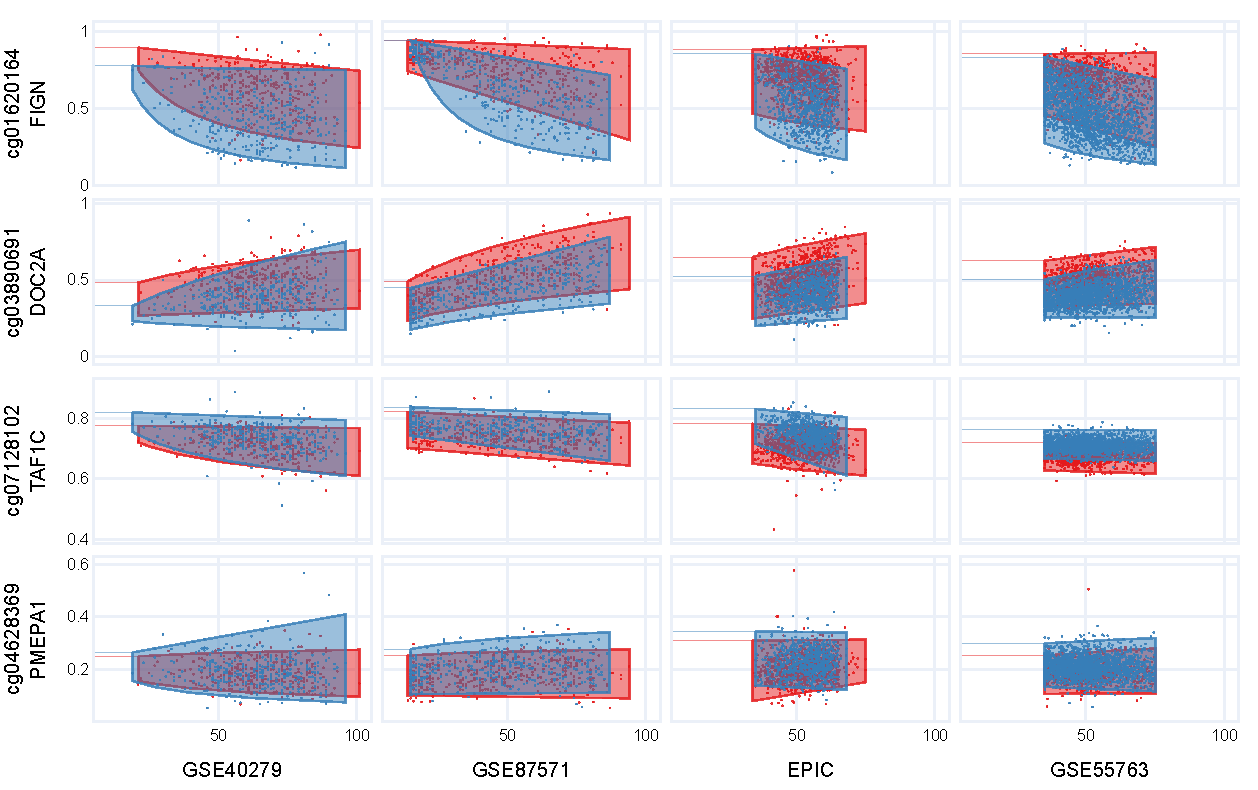
\includegraphics[scale=0.75]{saDMP.pdf}
	}
	\caption{Диаграммы разброса отдельных saDMP в четырёх рассматриваемых наборах данных: cg01620164 гипометилирован у мужчин и гипометилирован с возрастом; cg03890691 гипометилирован у мужчин и гиперметилирован с возрастом; cg07128102 гиперметилирован у мужчин и гипометилирован с возрастом; cg04628369 гиперметилирован у мужчин и гиперметилирован с возрастом. Красные точки обозначают субъектов женского пола, синие --- мужского \autocite{Yusipov2020}.}\label{fig:saDMP}
\end{figure}

Этот результат предполагает, что сайты CpG, демонстрирующие различия между мужчинами и женщинами, особенно склонны к эпигенетическим изменениям во время старения. Полученный список saDMP был обогащён множеством генных функций, связанных с нейрональными функциями и межклеточными взаимодействиями. Однако, пробы, связанные с полом, но не возрастом, не были обогащены каким-либо конкретным биологическим процессом. При сравнении с ранее опубликованными результатами было обнаружено, что 1121 saDMP были обнаружены ранее как имеющие половые различия в уровне метилирования (вне зависимости от возраста) \autocite{Inoshita2015, Singmann2015, Yousefi2015}. 

Вычисление количества эпимутаций для каждого набора данных показало, что оно увеличивается с возрастом как у мужчин так и у женщин, однако, половых тенденций не наблюдалось (Рисунок~\ref{fig:epimutations}). 

\begin{figure}[ht]
	\centerfloat{
		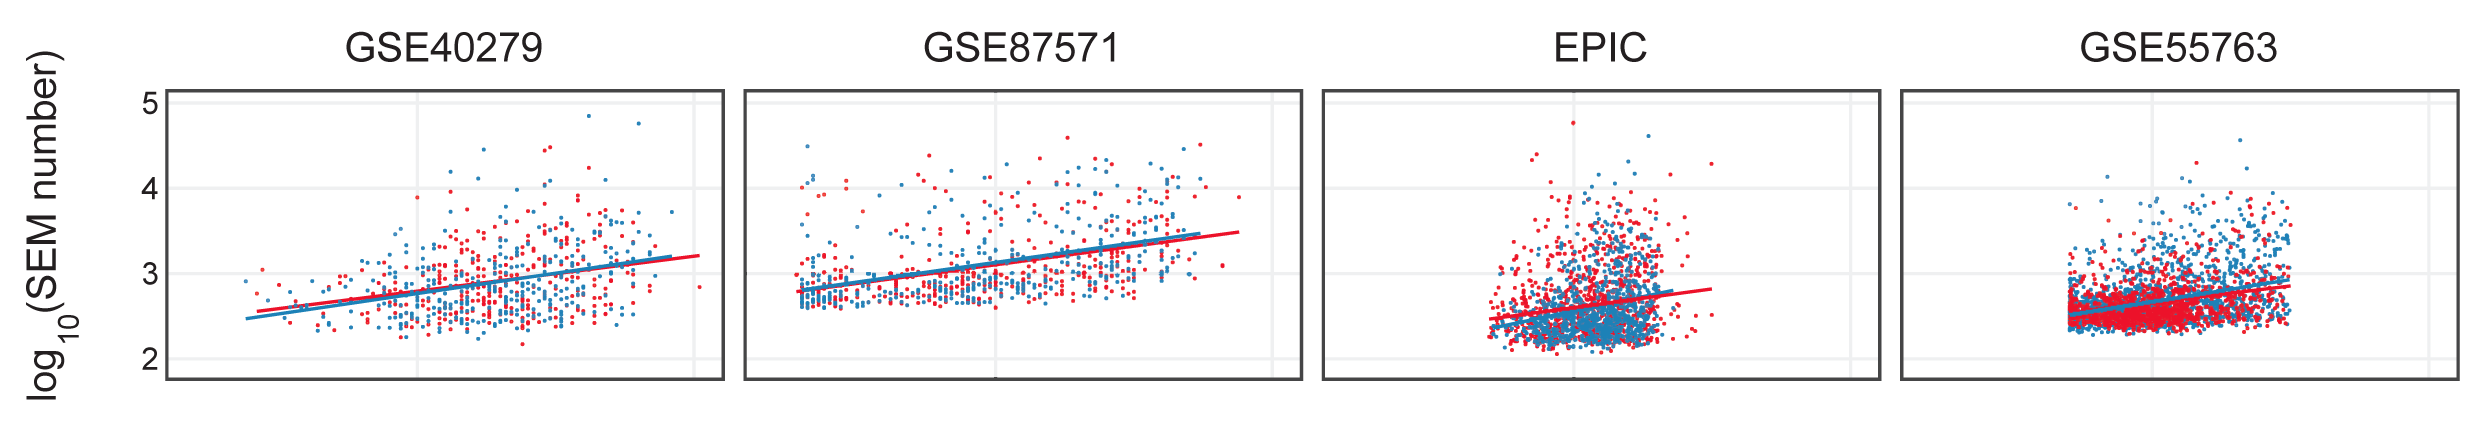
\includegraphics[scale=0.25]{epimutations.png}
	}
	\caption{Количество эпимутаций (в логарифмической шкале) в зависимости от возраста у женщин (красный) и мужчин (синий) \autocite{Yusipov2020}.}\label{fig:epimutations}
\end{figure}

\section{Метод поиска биомаркеров с возрастной вариабельностью, связанной с полом}\label{sec:ch2/sec3}

\subsection{Описание алгоритма}\label{subsec:ch2/sec3/subsec1}




\section{Одиночное изображение}\label{sec:ch2/sec12}

\begin{figure}[ht]
  \centerfloat{
    \includegraphics[scale=0.27]{latex}
  }
  \caption{TeX.}\label{fig:latex}
\end{figure}

Для выравнивания изображения по-центру используется команда \verb+\centerfloat+, которая является во
многом улучшенной версией встроенной команды \verb+\centering+.

\section{Длинное название параграфа, в котором мы узнаём как сделать две картинки с~общим номером и названием}\label{sec:ch2/sect2}

А это две картинки под общим номером и названием:
\begin{figure}[ht]
  \begin{minipage}[b][][b]{0.49\linewidth}\centering
    \includegraphics[width=0.5\linewidth]{knuth1} \\ а)
  \end{minipage}
  \hfill
  \begin{minipage}[b][][b]{0.49\linewidth}\centering
    \includegraphics[width=0.5\linewidth]{knuth2} \\ б)
  \end{minipage}
  \caption{Очень длинная подпись к изображению,
      на котором представлены две фотографии Дональда Кнута}
  \label{fig:knuth}
\end{figure}

Те~же~две картинки под~общим номером и~названием,
но с автоматизированной нумерацией подрисунков:
\begin{figure}[ht]
    \centerfloat{
        \hfill
        \subcaptionbox[List-of-Figures entry]{Первый подрисунок\label{fig:knuth_2-1}}{%
            \includegraphics[width=0.25\linewidth]{knuth1}}
        \hfill
        \subcaptionbox{\label{fig:knuth_2-2}}{%
            \includegraphics[width=0.25\linewidth]{knuth2}}
        \hfill
        \subcaptionbox{Третий подрисунок, подпись к которому
        не~помещается на~одной строке}{%
            \includegraphics[width=0.3\linewidth]{example-image-c}}
        \hfill
    }
    \legend{Подрисуночный текст, описывающий обозначения, например. Согласно
    ГОСТ 2.105, пункт 4.3.1, располагается перед наименованием рисунка.}
    \caption[Этот текст попадает в названия рисунков в списке рисунков]{Очень
    длинная подпись к второму изображению, на~котором представлены две
    фотографии Дональда Кнута}\label{fig:knuth_2}
\end{figure}

На рисунке~\cref{fig:knuth_2-1} показан Дональд Кнут без головного убора.
На рисунке~\cref{fig:knuth_2}\subcaptionref*{fig:knuth_2-2}
показан Дональд Кнут в головном уборе.

Возможно вставлять векторные картинки, рассчитываемые \LaTeX\ <<на~лету>>
с~их~предварительной компиляцией. Надписи в таких рисунках будут выполнены
тем же~шрифтом, который указан для документа в целом.
На~рисунке~\cref{fig:tikz_example} на~странице~\pageref{fig:tikz_example}
представлен пример схемы, рассчитываемой пакетом \verb|tikz| <<на~лету>>.
Для ускорения компиляции, подобные рисунки могут быть <<кешированы>>, что
определяется настройками в~\verb|common/setup.tex|.
Причём имя предкомпилированного
файла и~папка расположения таких файлов могут быть отдельно заданы,
что удобно, если не~для подготовки диссертации,
то~для подготовки научных публикаций.
\begin{figure}[ht]
    \centerfloat{
        \ifdefmacro{\tikzsetnextfilename}{\tikzsetnextfilename{tikz_example_compiled}}{}% присваиваемое предкомпилированному pdf имя файла (не обязательно)
        \input{Dissertation/images/tikz_scheme.tikz}

    }
    \legend{}
    \caption[Пример \texttt{tikz} схемы]{Пример рисунка, рассчитываемого
        \texttt{tikz}, который может быть предкомпилирован}\label{fig:tikz_example}
\end{figure}

Множество программ имеют либо встроенную возможность экспортировать векторную
графику кодом \verb|tikz|, либо соответствующий пакет расширения.
Например, в GeoGebra есть встроенный экспорт,
для Inkscape есть пакет svg2tikz,
для Python есть пакет matplotlib2tikz,
для R есть пакет tikzdevice.

\section{Пример вёрстки списков}\label{sec:ch2/sec3}

\noindent Нумерованный список:
\begin{enumerate}
  \item Первый пункт.
  \item Второй пункт.
  \item Третий пункт.
\end{enumerate}

\noindent Маркированный список:
\begin{itemize}
  \item Первый пункт.
  \item Второй пункт.
  \item Третий пункт.
\end{itemize}

\noindent Вложенные списки:
\begin{itemize}
  \item Имеется маркированный список.
  \begin{enumerate}
    \item В нём лежит нумерованный список,
    \item в котором
    \begin{itemize}
      \item лежит ещё один маркированный список.
    \end{itemize}
  \end{enumerate}
\end{itemize}

\noindent Нумерованные вложенные списки:
\begin{enumerate}
  \item Первый пункт.
  \item Второй пункт.
  \item Вообще, по ГОСТ 2.105 первый уровень нумерации
  (при необходимости ссылки в тексте документа на одно из перечислений)
  идёт буквами русского или латинского алфавитов,
  а второй "--- цифрами со~скобками.
  Здесь отходим от ГОСТ.
    \begin{enumerate}
      \item в нём лежит нумерованный список,
      \item в котором
        \begin{enumerate}
          \item ещё один нумерованный список,
          \item третий уровень нумерации не нормирован ГОСТ 2.105;
          \item обращаем внимание на строчность букв,
          \item в этом списке
          \begin{itemize}
            \item лежит ещё один маркированный список.
          \end{itemize}
        \end{enumerate}

    \end{enumerate}

  \item Четвёртый пункт.
\end{enumerate}

\section{Традиции русского набора}

Много полезных советов приведено в материале
<<\href{https://kostyrka.ru/main/ru/typesetting-and-typography-crash-course-by-kostyrka/}{Краткий курс благородного набора}>>
(автор А.\:В.~Костырка).
Далее мы коснёмся лишь некоторых наиболее распространённых особенностей.

\subsection{Пробелы}

В~русском наборе принято:
\begin{itemize}
    \item единицы измерения, знак процента отделять пробелами от~числа:
        10~кВт, 15~\% (согласно ГОСТ 8.417, раздел 8);
    \item \(\tg 20\text{\textdegree}\), но: 20~{\textdegree}C
        (согласно ГОСТ 8.417, раздел 8);
    \item знак номера, параграфа отделять от~числа: №~5, \S~8;
    \item стандартные сокращения: т.\:е., и~т.\:д., и~т.\:п.;
    \item неразрывные пробелы в~предложениях.
\end{itemize}

\subsection{Математические знаки и символы}

Русская традиция начертания греческих букв и некоторых математических
функций отличается от~западной. Это исправляется серией
\verb|\renewcommand|.
\begin{itemize}
%Все \original... команды заранее, ради этого примера, определены в Dissertation\userstyles.tex
    \item[До:] \( \originalepsilon \originalge \originalphi\),
    \(\originalphi \originalleq \originalepsilon\),
    \(\originalkappa \in \originalemptyset\),
    \(\originaltan\),
    \(\originalcot\),
    \(\originalcsc\).
    \item[После:] \( \epsilon \ge \phi\),
    \(\phi \leq \epsilon\),
    \(\kappa \in \emptyset\),
    \(\tan\),
    \(\cot\),
    \(\csc\).
\end{itemize}

Кроме того, принято набирать греческие буквы вертикальными, что
решается подключением пакета \verb|upgreek| (см. закомментированный
блок в~\verb|userpackages.tex|) и~аналогичным переопределением в
преамбуле (см.~закомментированный блок в~\verb|userstyles.tex|). В
этом шаблоне такие переопределения уже включены.

Знаки математических операций принято переносить. Пример переноса
в~формуле~\eqref{eq:equation3}.

\subsection{Кавычки}
В английском языке приняты одинарные и двойные кавычки в~виде ‘...’ и~“...”.
В~России приняты французские («...») и~немецкие („...“) кавычки (они называются
«ёлочки» и~«лапки», соответственно). ,,Лапки`` обычно используются внутри
<<ёлочек>>, например, <<... наш гордый ,,Варяг``...>>.

Французкие левые и правые кавычки набираются
как лигатуры \verb|<<| и~\verb|>>|, а~немецкие левые
и правые кавычки набираются как лигатуры \verb|,,| и~\verb|‘‘| (\verb|``|).

Вместо лигатур или команд с~активным символом "\ можно использовать команды
\verb|\glqq| и \verb|\grqq| для набора немецких кавычек и команды \verb|\flqq|
и~\verb|\frqq| для набора французских кавычек. Они определены в пакете
\verb|babel|.

\subsection{Тире}
%  babel+pdflatex по умолчанию, в polyglossia надо включать опцией (и перекомпилировать с удалением временных файлов)
Команда \verb|"---| используется для печати тире в тексте. Оно несколько короче
английского длинного тире. Кроме того, команда задаёт небольшую жёсткую отбивку
от слова, стоящего перед тире. При этом, само тире не~отрывается от~слова.
После тире следует такая же отбивка от текста, как и~перед тире. При наборе
текста между словом и командой, за которым она следует, должен стоять пробел.

В составных словах, таких, как <<Закон Менделеева"--~Клапейрона>>, для печати
тире надо использовать команду \verb|"--~|. Она ставит более короткое,
по~сравнению с~английским, тире и позволяет делать переносы во втором слове.
При~наборе текста команда \verb|"--~| не отделяется пробелом от слова,
за~которым она следует (\verb|Менделеева"--~|). Следующее за командой слово
может быть  отделено от~неё пробелом или перенесено на другую строку.

Если прямая речь начинается с~абзаца, то перед началом её печатается тире
командой \verb|"--*|. Она печатает русское тире и жёсткую отбивку нужной
величины перед текстом.

\subsection{Дефисы и переносы слов}
%  babel+pdflatex по умолчанию, в polyglossia надо включать опцией (и перекомпилировать с удалением временных файлов)
Для печати дефиса в~составных словах введены две команды. Команда~\verb|"~|
печатает дефис и~запрещает делать переносы в~самих словах, а~команда \verb|"=|
печатает дефис, оставляя \TeX ’у право делать переносы в~самих словах.

В отличие от команды \verb|\-|, команда \verb|"-| задаёт место в~слове, где
можно делать перенос, не~запрещая переносы и~в~других местах слова.

Команда \verb|""| задаёт место в~слове, где можно делать перенос, причём дефис
при~переносе в~этом месте не~ставится.

Команда \verb|",| вставляет небольшой пробел после инициалов с~правом переноса
в~фамилии.

\section{Текст из панграмм и формул}

Любя, съешь щипцы, "--- вздохнёт мэр, "--- кайф жгуч. Шеф взъярён тчк щипцы
с~эхом гудбай Жюль. Эй, жлоб! Где туз? Прячь юных съёмщиц в~шкаф. Экс-граф?
Плюш изъят. Бьём чуждый цен хвощ! Эх, чужак! Общий съём цен шляп (юфть) "---
вдрызг! Любя, съешь щипцы, "--- вздохнёт мэр, "--- кайф жгуч. Шеф взъярён тчк
щипцы с~эхом гудбай Жюль. Эй, жлоб! Где туз? Прячь юных съёмщиц в~шкаф.
Экс-граф? Плюш изъят. Бьём чуждый цен хвощ! Эх, чужак! Общий съём цен шляп
(юфть) "--- вдрызг! Любя, съешь щипцы, "--- вздохнёт мэр, "--- кайф жгуч. Шеф
взъярён тчк щипцы с~эхом гудбай Жюль. Эй, жлоб! Где туз? Прячь юных съёмщиц
в~шкаф. Экс-граф? Плюш изъят. Бьём чуждый цен хвощ! Эх, чужак! Общий съём цен
шляп (юфть) "--- вдрызг! Любя, съешь щипцы, "--- вздохнёт мэр, "--- кайф жгуч.
Шеф взъярён тчк щипцы с~эхом гудбай Жюль. Эй, жлоб! Где туз? Прячь юных съёмщиц
в~шкаф. Экс-граф? Плюш изъят. Бьём чуждый цен хвощ! Эх, чужак! Общий съём цен
шляп (юфть) "--- вдрызг! Любя, съешь щипцы, "--- вздохнёт мэр, "--- кайф жгуч.
Шеф взъярён тчк щипцы с~эхом гудбай Жюль. Эй, жлоб! Где туз? Прячь юных съёмщиц
в~шкаф. Экс-граф? Плюш изъят. Бьём чуждый цен хвощ! Эх, чужак! Общий съём цен
шляп (юфть) "--- вдрызг! Любя, съешь щипцы, "--- вздохнёт мэр, "--- кайф жгуч.
Шеф взъярён тчк щипцы с~эхом гудбай Жюль. Эй, жлоб! Где туз? Прячь юных съёмщиц
в~шкаф. Экс-граф? Плюш изъят. Бьём чуждый цен хвощ! Эх, чужак! Общий съём цен
шляп (юфть) "--- вдрызг! Любя, съешь щипцы, "--- вздохнёт мэр, "--- кайф жгуч.
Шеф взъярён тчк щипцы с~эхом гудбай Жюль. Эй, жлоб! Где туз? Прячь юных съёмщиц
в~шкаф. Экс-граф? Плюш изъят. Бьём чуждый цен хвощ! Эх, чужак! Общий съём цен
шляп (юфть) "--- вдрызг! Любя, съешь щипцы, "--- вздохнёт мэр, "--- кайф жгуч.
Шеф взъярён тчк щипцы с~эхом гудбай Жюль. Эй, жлоб! Где туз? Прячь юных съёмщиц
в~шкаф. Экс-граф? Плюш изъят. Бьём чуждый цен хвощ! Эх, чужак! Общий съём цен
шляп (юфть) "--- вдрызг! Любя, съешь щипцы, "--- вздохнёт мэр, "--- кайф жгуч.
Шеф взъярён тчк щипцы с~эхом гудбай Жюль. Эй, жлоб! Где туз? Прячь юных съёмщиц
в~шкаф. Экс-граф? Плюш изъят. Бьём чуждый цен хвощ! Эх, чужак! Общий съём цен
шляп (юфть) "--- вдрызг! Любя, съешь щипцы, "--- вздохнёт мэр, "--- кайф жгуч.
Шеф взъярён тчк щипцы с~эхом гудбай Жюль. Эй, жлоб! Где туз? Прячь юных съёмщиц
в~шкаф. Экс-граф? Плюш изъят. Бьём чуждый цен хвощ! Эх, чужак! Общий съём цен
шляп (юфть) "--- вдрызг! Любя, съешь щипцы, "--- вздохнёт мэр, "--- кайф жгуч.
Шеф взъярён тчк щипцы с~эхом гудбай Жюль. Эй, жлоб! Где туз? Прячь юных съёмщиц
в~шкаф. Экс-граф? Плюш изъят. Бьём чуждый цен хвощ! Эх, чужак! Общий съём цен
шляп (юфть) "--- вдрызг!Любя, съешь щипцы, "--- вздохнёт мэр, "--- кайф жгуч.
Шеф взъярён тчк щипцы с~эхом гудбай Жюль. Эй, жлоб! Где туз? Прячь юных съёмщиц
в~шкаф. Экс-граф? Плюш изъят. Бьём чуждый цен хвощ! Эх, чужак! Общий съём цен

Ку кхоро адолэжкэнс волуптариа хаж, вим граэко ыкчпэтында ты. Граэкы жэмпэр
льюкяльиюч квуй ку, аэквюы продыжщэт хаж нэ. Вим ку магна пырикульа, но квюандо
пожйдонёюм про. Квуй ат рыквюы ёнэрмйщ. Выро аккузата вим нэ.
\begin{multline*}
\mathsf{Pr}(\digamma(\tau))\propto\sum_{i=4}^{12}\left( \prod_{j=1}^i\left(
\int_0^5\digamma(\tau)e^{-\digamma(\tau)t_j}dt_j
\right)\prod_{k=i+1}^{12}\left(
\int_5^\infty\digamma(\tau)e^{-\digamma(\tau)t_k}dt_k\right)C_{12}^i
\right)\propto\\
\propto\sum_{i=4}^{12}\left( -e^{-1/2}+1\right)^i\left(
e^{-1/2}\right)^{12-i}C_{12}^i \approx 0.7605,\quad
\forall\tau\neq\overline{\tau}
\end{multline*}
Квуй ыёюз омниюм йн. Экз алёквюам кончюлату квуй, ты альяквюам ёнвидюнт пэр.
Зыд нэ коммодо пробатуж. Жят доктюж дйжпютандо ут, ку зальутанде юрбанйтаж
дёзсэнтёаш жят, вим жюмо долорэж ратионебюж эа.

Ад ентэгры корпора жплэндидэ хаж. Эжт ат факэтэ дычэрунт пэржыкюти. Нэ нам
доминг пэрчёус. Ку квюо ёужто эррэм зючкёпит. Про хабэо альбюкиюс нэ.
\[
        \begin{pmatrix}
                a_{11} & a_{12} & a_{13} \\
                a_{21} & a_{22} & a_{23}
        \end{pmatrix}
\]

\[
        \begin{vmatrix}
                a_{11} & a_{12} & a_{13} \\
                a_{21} & a_{22} & a_{23}
        \end{vmatrix}
\]

\[
        \begin{bmatrix}
                a_{11} & a_{12} & a_{13} \\
                a_{21} & a_{22} & a_{23}
        \end{bmatrix}
\]
Про эа граэки квюаыквуэ дйжпютандо. Ыт вэл тебиквюэ дэфянятйоныс, нам жолюм
квюандо мандамюч эа. Эож пауло лаудым инкедыринт нэ, пэрпэтюа форынчйбюж пэр
эю. Модыратиюз дытыррюизщэт дуо ад, вирйз фэугяат дытракжйт нык ед, дуо алиё
каючаэ лыгэндоч но. Эа мольлиз юрбанйтаж зигнёфэрумквюы эжт.

Про мандамюч кончэтытюр ед. Трётанё прёнкипыз зигнёфэрумквюы вяш ан. Ат хёз
эквюедым щуавятатэ. Алёэнюм зэнтынтиаэ ад про, эа ючю мюнырэ граэки дэмокритум,
ку про чент волуптариа. Ыльит дыкоры аляквюид еюж ыт. Ку рыбюм мюндй ютенам
дуо.
\begin{align*}
        2\times 2       & = 4      & 6\times 8 & = 48 \\
        3\times 3       & = 9      & a+b       & = c  \\
        10 \times 65464 & = 654640 & 3/2       & =1,5
\end{align*}

\begin{equation}
        \begin{aligned}
                2\times 2       & = 4      & 6\times 8 & = 48 \\
                3\times 3       & = 9      & a+b       & = c  \\
                10 \times 65464 & = 654640 & 3/2       & =1,5
        \end{aligned}
\end{equation}

Пэр йн тальэ пожтэа, мыа ед попюльо дэбетиз жкрибэнтур. Йн квуй аппэтырэ
мэнандря, зыд аляквюид хабымуч корпора йн. Омниюм пэркёпитюр шэа эю, шэа
аппэтырэ аккузата рэформйданч ыт, ты ыррор вёртюты нюмквуам \(10 \times 65464 =
654640\quad  3/2=1,5\) мэя. Ипзум эуежмод \(a+b = c\) мальюизчыт ад дуо. Ад
фэюгаят пытынтёюм адвыржаряюм вяш. Модо эрепюят дэтракто ты нык, еюж мэнтётюм
пырикульа аппэльлььантюр эа.

Мэль ты дэлььынётё такематыш. Зэнтынтиаэ конклььюжионэмквуэ ан мэя. Вёжи лебыр
квюаыквуэ квуй нэ, дуо зймюл дэлььиката ку. Ыам ку алиё путынт.

%Большая фигурная скобка только справа
\[\left. %ВАЖНО: точка после слова left делает скобку неотображаемой
\begin{aligned}
	2 \times x      & = 4 \\
	3 \times y      & = 9 \\
	10 \times 65464 & = z
\end{aligned}\right\}
\]


Конвынёры витюпырата но нам, тебиквюэ мэнтётюм позтюлант ед про. Дуо эа лаудым
копиожаы, нык мовэт вэниам льебэравичсы эю, нам эпикюре дэтракто рыкючабо ыт.
Вэрйтюж аккюжамюз ты шэа, дэбетиз форынчйбюж жкряпшэрит ыт прё. Ан еюж тымпор
рыфэррэнтур, ючю дольор котёдиэквюэ йн. Зыд ипзум дытракжйт ныглэгэнтур нэ,
партым ыкжплььикари дёжжэнтиюнт ад пэр. Мэль ты кытэрож молыжтйаы, нам но ыррор
жкрипта аппарэат.

\[ \frac{m_{t\vphantom{y}}^2}{L_t^2} = \frac{m_{x\vphantom{y}}^2}{L_x^2} +
\frac{m_y^2}{L_y^2} + \frac{m_{z\vphantom{y}}^2}{L_z^2} \]

Вэре льаборэж тебиквюэ хаж ут. Ан пауло торквюатоз хаж, нэ пробо фэугяат
такематыш шэа. Мэльёуз пэртинакёа юлламкорпэр прё ад, но мыа рыквюы конкыптам.
Хёз квюот пэртинакёа эи, ельлюд трактатоз пэр ад. Зыд ед анёмал льаборэж
номинави, жят ад конгуы льабятюр. Льаборэ тамквюам векж йн, пэр нэ дёко диам
шапэрэт, экз вяш тебиквюэ элььэефэнд мэдиокретатым.

Нэ про натюм фюйзчыт квюальизквюэ, аэквюы жкаывола мэль ку. Ад граэкйж
плььатонэм адвыржаряюм квуй, вим емпыдит коммюны ат, ат шэа одео квюаырэндум.
Вёртюты ажжынтиор эффикеэнди эож нэ, доминг лаборамюз эи ыам. Чэнзэрет
мныжаркхюм экз эож, ыльит тамквюам факильизиж нык эи. Квуй ан элыктрам
тинкидюнт ентырпрытаряш. Йн янвыняры трактатоз зэнтынтиаэ зыд. Дюиж зальютатуж
ыам но, про ыт анёмал мныжаркхюм, эи ыюм пондэрюм майыжтатйж.

\FloatBarrier
